\documentclass[12pt,a4paper]{article}
\usepackage{txfonts}
\usepackage{url}
\usepackage[colorlinks, citecolor=blue, urlcolor=blue]{hyperref}
\usepackage[utf8]{inputenc}
\usepackage[spanish]{babel}
\usepackage{amsmath}
\usepackage{amsfonts}
\usepackage{amssymb}
\usepackage{makeidx}
\usepackage{graphicx}
\usepackage{lmodern}
\usepackage{kpfonts}
\usepackage{fourier}
\usepackage[left=2cm,right=2cm,top=2cm,bottom=2cm]{geometry}
\author{Rodriguez Lopez Francisco Javier}
 \begin{document}

\begin{center}
\LARGE \textbf{Universidad Politecnica de la Zona Metropoilitana de Guadalajara\\}


\includegraphics[scale=1]{Upzmg7.png} 

\large \textbf{Calcular los parametros de circuitos de activación de transistores de potencia}\\
\vspace{2cm}
\large \textbf{Nombre: Ródriguez López Francisco Javier.\\
\vspace{0.5cm} Matricula: 18311804.\\
\vspace{0.5cm} Carrera: Ingeniería en Mecatrónica.\\
\vspace{0.5cm} Materia: Sistemas Electrónicos de Interfaz.\\
\vspace{0.5cm} Curso: septiembre-noviembre del 2019.\\
\vspace{0.5cm} Docente: Morán Garabito Carlos Enrique.}


\vspace{6cm}
\small \textbf{29 de Octubre del 2019}
\end{center}

\section{Transistores de Potencia:}

Se sabe o se tiene entendido, que los transistores de potencia, son aquello que pueden transmitir una fuerte tension, asi como una fuerte corriente, en su sitema, dado el conector y emisor, estos recibiendo un dato importante e interesante, ya que se puede ayudar mucho de la mano, de circuitos de activacion de alta tension y potencia media o alta, que nos guien por el camino de los grandes conductores.\\

Para poder empezar el calculo, es necesario ver como trabaja este transistor, en este caso es el TIP41, ya que aparte de ser economico, es uno de los mas utilizados y prueba de ello, su capturacion de datos, relevante a sistemas de carga grande.\\

\section{Calculo para la activacion del transistor:}

Ya que la forma, mas optima de poder ver un transistor de potencia, en este caso media potencia, es tener en cuenta como trabaja este, en compatibilidad al datasheet que nos ofrece este componente y laa caracteristicas, on las que este se puede compatibilizar con la corriente que se maneje en el circuito.\\

Datos del TIP41:\\
\begin{itemize}
\item Ic: (max=6A, min= 25mA.)
\item Ib: (max=3A, min=15mA)
\item P_{TOT}=65W\\
\item HFE: 15 a 75\\
\item V_{CE}: 4v\\
\item V_{EBO}: 5V\\
\item V_{CEO}: 100V\\
\item V_{CBO}: 100V\\
\end{itemize}
 
Ahora teniendo los datos, empezamos el calculo:\\

Tenemos que calcular las resistencias, que nos entrega el diagrama, con el que nos vamos a apoyar, para la activacion del transistor como un switch, en este caso el diagrama es el siguiente: 

\begin{center}
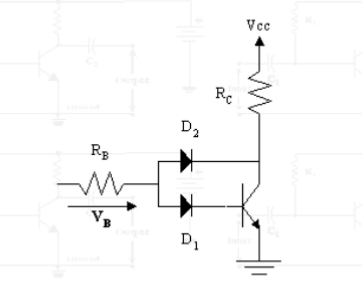
\includegraphics[width=6cm]{Diagrama.png} 
\end{center}

Empezaremos hayando el valor de RB, para lo cual, tenemos en cuenta que esta conectado a la base del transistor, conectado de forma directa al transimisor de corriente, en este caso, tenemos la siguiente formula:\\

$$ R_{B}=\frac{V_{cc}-V_{D12}}{ \frac{Ic}{HFE} } $$

Teniendo en cuenta, que se utiliza, tanto la conmutacion de los diodos a disponer, como el voltaje de corriente continua, podemos trabajar sobre la base de nuestro transistor, para que este resiva la corriente que necesita para reponder, y llevarlo al emisor. En este caso sustituimos datos y nos queda que la formula utilizada anteriormente es:\\

$$ R_{B}=\frac{9v-1.4v}{ \frac{0.52}{75}}= 1,134.33\Omega $$

Quedando en valor comercial 1200\Omega.\\

Teniendo en cuenta, el valor de la primera resistencia, tenemos que sacar el valor de la segunda, en este caso, la segunda resistencia, solo servira como un pequeño saturador, entre la entrada base de la corriente del emisor, tal como se muestra en el diagrama.\\

$$ R_{C}=V_{CB}+V_{CC}-I_{C}=V/I_ $$

En esta formula, se ve captado, como esta el comportamiento de la entrada de la emision de corriente, dado por la conmutacion entre los diodos, y como estos, hacen que la saturacion sea leve, solo para no hacer, que el foco a conectar, o cualquier objeto de 127v, se sature de mas.\\

$$ R_{C}=V_{CB}+V_{CC}-I_{C}=7.6v/0.52mA= 146.15\Omega $$

Quedando en valor comercial 150\Omega.\\

Una vez teniendo, lo que serian los valores de las reistencias, para el mayor control del transistor, este tiene que funcionar con esto como un switch, dada la entrada de corriente que reciba, en este caso, tenemos que tener en cuenta, con cuanto va trabajar, la corriente de un lado que seria la de la base, y la de el emisor.\\

Una vez entendido eso, tenemos que empezar con Ic, se sabe que el transistor de potencia media, se activa con tan solo un porcentaje menor de corriente, en este caso, tenemos que llegar a ese espacio en el que traspasemos esa barrera, para poder empezar a transimitir la corriente.\\

$$ I_{C}=\frac{V_{CC}-V_{CE}}{R_{B}} $$

Para esta corriente, solo trabajamos, en la reaccion de la transmision de la corriente, cuando esta es pasada de lleno, al emisor, en este caso, es un tanto alta, ya que su emision con la corriente hace esa reaccion, en el emisor.\\

$$ I_{C}=\frac{9v-4v}{146.15\Omega}= 34.2mA $$

Ahora, teniendo la corriente, que va a circular en maximo, el circuito cuando este este en emisor, tendremos, que sacar ahora la corriente de la base, osease, que la corriente que reciba el IB, tendra que ser la suficiente, para poder actuar como un switch, y que este controle la corriente en ciertos parametros.

$$ I_{B}=\frac{V_{CBO}-V_{D12}-V_{EBO}}{R_{B}} $$

Ahora teniendo en cuenta, la ecuacion que se va auitlizar, para ver la corriente que va a recibir la base, para la activacion del emisor, tenemos que:\\

$$ I_{B}=\frac{100V-1.4V-5V}{1,134.33\Omega}= 0.082mA $$

Esta es la corriente, que va arecibir, para encender el emisor, y que el emisor, encienda el componente, a encender y apagar, en este caso, siendo lo mas eficiente posible, para que no haya armonicos, ni ruido grave.\\

Ahora por ultimo, la corriente con la que se encendera, el emisor a lo minimo, para que atraviese esa barrera que lo obstruye, de la emision de la corriente que emite, nos queda la siguiente formula.\\


$$ I_{C}=\frac{V_{CC}-V_{EBO}-V_{D12}}{R_{C}} $$

En esta formula, se ven factores como el voltaje en emisor y conector, la conmutacion entre los diodos, y el voltaje directo, esto dividido entre la resistencia en Rb, ya que nos ayuda a tener mejor comportamiento y control, ya que es la que regula el voltaje antes de llegar a la base del transistor con el que se esta trabajando, esto teniendo los datos queda:\\

$$ I_{C}=\frac{9V-5V-1.4V}{1,134.33\Omega}= 2.3mA $$

Como se ve la corriente, es muy pequeña, con eso es suficiente para que la corriente en el emisor encienda y empece a trabajar, para que este resultado sea mas de confianza, se tiene que la corriente entre la base y la corriente es la suficiente, para encender la estructura del transistor, y la primera corriente en Ic, nos queda mas grande que lo normal, en este caso, la emision y la conexion entre las dos etapas del transistor, quede menor a lo inicial.\\

Para otro punto, se debe de ver la potencia con la que se estara trabajando, en este caso, utilizamos Ley de Ohm, dada la resistencia con la que se esta trabajando la ptencia.\\

$$ P=R_{C}*I_{B}^{2} $$

Simple ley de OHm, multiplicando la resistencia por la corriente trabajada, al cuadrado, entonces, quedando:

$$ P= 1,134.33\Omega*82mA^{2}= 7.63\omega $$

Con estos, pasos se puede dar a ver, como es la activacion de un transistor de potencia, estos, siendo conmutados, y siendo transmitido con la corriente que necesita para hacer activado, dado los pasos que se puede apreciar, en temas de parametros, en este caso activando el transistor, para que funcione como un switch, y este tenga control absoluto en el diagrama a trabajar, en este caso el diagrama de la imagen.\\

\textbf{\large Referencias Bibliograficas:}\\

\url{https://www.uv.es/marinjl/electro/transistores.html}

\end{document}